\documentclass[letterpaper,10pt,conference]{ieeeconf}
\IEEEoverridecommandlockouts
\overrideIEEEmargins
\usepackage{fontspec}
\setmainfont{Times New Roman}\setsansfont{Arial}\setmonofont{Menlo}
\usepackage{amsmath,amssymb,graphicx,booktabs,cite,url}
\graphicspath{{figures/}}
\newcommand{\vct}[1]{\vec{#1}}
\newcommand{\BudgetSpeed}{$0.283\,\mathrm{m/s}$}
\newcommand{\WalkSpeed}{$0.126\,\mathrm{m/s}$}
\newcommand{\AbstractRateResult}{The maximum sector-command rate decreases from 1517 to 536 degree/s relative to the original allocator, retaining 99.95\% of its mean forward speed.}

\title{\LARGE\bf Rewind-Aware Rolling Allocation\\for an Articulated Arc-Leg Hexapod}
\author{\mbox{}}
\begin{document}
\maketitle\thispagestyle{empty}\pagestyle{empty}
\begin{abstract}
A finite-arc leg with bounded distal rotation must periodically rewind its rolling motion. Limiting stance rotation by the arc geometry alone can leave too little swing time for a rate-bounded rewind. We present a rolling allocator that limits sector excursion by the available swing time, anticipates the next reindexing opportunity, and assigns the remaining contact travel to articulation. The sector command satisfies a discrete rate bound; this bound does not constrain the summed inverse-kinematics and sector target. We evaluate the method on an eighteen-actuator hexapod in 268 prescribed MuJoCo trials. At a 0.45 m/s forward command, the method reduces the largest sector-command rate from 1517 to 536 degree/s while retaining 99.95\% of the original allocator's mean speed of 0.283 m/s. The largest summed distal-target rate also decreases, from 3300 to 1406 degree/s, but remains above the sector bound. Periodic reindexing achieves comparable transport, so the evidence supports rewind-aware allocation without establishing an advantage for adaptive scheduling. These results characterize a simulation-based control mechanism; quantitative validation of the proposed controller on hardware remains open.
\end{abstract}

\section{INTRODUCTION}
An articulated leg ending in a finite circular arc can move through both rolling and joint articulation. With a bounded distal joint, the arc eventually reaches an orientation from which it must be lifted and rewound. The controller must therefore reserve enough swing time to restore the arc before its next stance. This constraint matters even when the robot moves successfully: a rewind without an explicit rate constraint may preserve body speed while demanding abrupt distal motion.

The relevant limit is temporal as well as geometric. At a swing duration of 0.20 s and a sector-rate budget of $540^\circ$/s, a rest-to-rest quintic rewind can recover only $57.6^\circ$, despite a geometric excursion of $100^\circ$. Figure~\ref{fig:overview} illustrates this mismatch and the measured effect of limiting rewind demand. Reducing the allowed rotation also changes how much contact travel the articulated joints must supply. A sector bound can consequently make a previously reachable stance trajectory infeasible unless the controller also schedules reindexing and reallocates the residual travel.

We couple these decisions in a position-target allocator. It assigns rolling roles from contact geometry, constrains sector excursion using swing time, reindexes before the next opportunity would be missed, and subtracts the realized rolling increment from the requested articulated motion. The analytical component is a sufficient sector-command bound for a specified interpolation profile. The empirical question is whether this constraint can be imposed without losing the transport supplied by rolling.

Our contributions are: (1) a swing-time constraint coupled to post-saturation contact-travel allocation, including an explicit statement of the sector-rate guarantee and its assumptions; and (2) a paired mechanism study that compares the complete rewind treatment with the original allocator, periodic reindexing, and component restrictions under one morphology. A concavity-preserving collision approximation supports the experiments. We treat curved legs and stride-level rolling/stepping as established ideas; neither the quintic interpolation nor the collision decomposition is claimed as a new method.

\begin{figure}[t]
\centering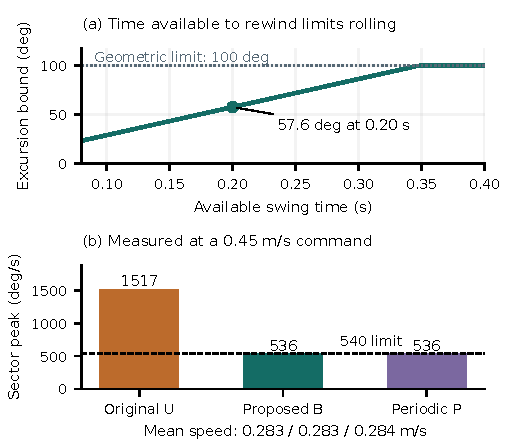
\includegraphics[width=\columnwidth]{overview.pdf}
\caption{The rewind constraint and its measured effect. (a) Analytical excursion bound for $\Omega=540^\circ$/s and a $100^\circ$ geometric limit. (b) Largest sector rates over eight initial phases; speeds are eight-trial means. U, B, and P all complete the 8 s trials. P shows that periodic reindexing is a competitive alternative. The dashed rate bound applies to the sector component only.}
\label{fig:overview}
\end{figure}

\section{RELATED WORK}
RHex established the mobility of a hexapod with continuously rotating compliant curved legs~\cite{saranli2001rhex}. Q-Whex further develops quasi-wheeled hexapod motion~\cite{zhang2023qwhex}. Energy-oriented design guidelines and kinematic studies also connect C-leg geometry to locomotion performance~\cite{vina2021cleg,burzynski2024kinematics}. These systems motivate efficient use of curved contacts, while the present problem concerns an arc mounted after two additional articulated joints and restricted to a bounded position range.

Transformable leg-wheel robots provide the closest morphological context. Quattroped shares actuation across wheel and leg configurations~\cite{chen2014quattroped}, and TurboQuad addresses smooth behavioral transitions~\cite{chen2017turboquad}. R-Taichi studies rolling and swing strategies on a transformable two-degree-of-freedom limb, including physical experiments~\cite{xue2025rolling}. Chang and Lin describe stride-level hybrid locomotion with aerial repositioning and energy-oriented optimization~\cite{chang2026stride}. Accordingly, combining rolling and swing within a stride is established. Our narrower question is how to bound the rotation of a fixed finite sector by its available rewind interval and allocate the remaining contact travel to articulation.

Articulated wheel-leg platforms also coordinate contact placement and rolling, including ASTERISK H~\cite{yoshioka2008asterisk}, whole-body wheeled-quadruped control~\cite{bjelonic2019keep}, and online gait-sequence generation with model predictive control~\cite{bjelonic2021wholebody}. These methods address broader force and motion planning problems. Our allocator uses geometric roles and position targets without online force optimization or learned policies. The experiments therefore test its internal mechanisms under a common embodiment and motor setup, rather than claim superiority over whole-body controllers on different robots.

Repeatable testing matters when small control changes alter contact sequences. Weng et al.~\cite{weng2024testing} demonstrate the importance of controlled conditions in legged-robot evaluation. We use fixed paired phases and explicit parameter stress conditions, report failures as well as transport, and distinguish these deterministic comparisons from hardware reliability estimates.

\section{PLATFORM AND CONTACT REPRESENTATION}
\subsection{Embodiment and Actuation}
The model is a hexapod with three revolute joints per leg and eighteen actuators. The first joint steers the limb about a vertical axis. The second and third joints articulate the leg, with the third joint also rotating the arc; there is no additional wheel actuator. The model mass is 4.161 kg. The tire envelope has an outer radius of 122.5 mm, an inner radius of 112.5 mm, and a width of 44 mm. Dimensions in the historical drawing provide manufacturing context but do not calibrate the compliance of the simulated tire.

Every condition uses the same floating base, inertias, controller gains, voltage limits, and nominal pose. The actuator path computes a proportional-derivative torque request and a bounded voltage command,
\begin{align}
 \tau_j^c&=k_{p,j}(q_j^\star-q_j)+k_{d,j}(\dot q_j^\star-\dot q_j),\\
 V_j&=\operatorname{sat}_{[-12,12]}[(R_j/K_j)\tau_j^c+K_j\dot q_j].
\end{align}
Reflected rotor inertia is included. The common gait setup disables the additional target-profile velocity and acceleration limiter and doubles the middle-joint proportional gain, with damping scaled by $\sqrt{2}$. Voltage and torque limits remain active. Thus the rate studied below is an explicit sector-command constraint, not a measured actuator capability or a guarantee on the total articulated joint rate.

\begin{figure}[t]
\centering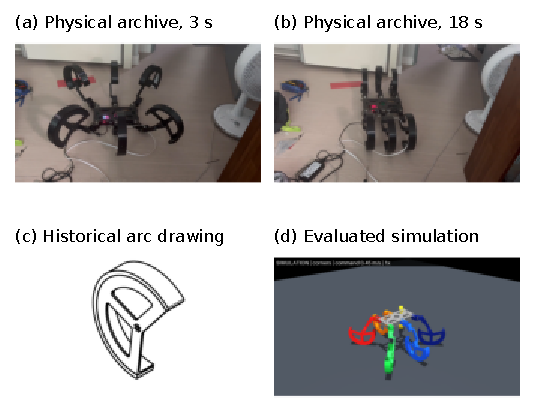
\includegraphics[width=\columnwidth]{platform.pdf}
\caption{SCONE embodiment and evaluated model. (a,b) Archival floor-motion frames at source times 3 and 18 s. (c) Historical arc fabrication drawing. (d) Nominal simulation pose. The physical clips use an undocumented earlier controller and include external cables; they do not validate the proposed allocator on hardware.}
\label{fig:platform}
\end{figure}

\subsection{Contact Geometry and Rolling Direction}
Let $\vct{a}_i$ be the distal axis, $\vct{o}_i$ a point on it, and $\vct{p}_{c,i}$ the geometric support centroid. The planar material velocity induced by unit distal rotation is
\begin{equation}
 \vct{t}_i=\vct{a}_i\times(\vct{p}_{c,i}-\vct{o}_i),\qquad
 r_i=\|\vct{t}_{i,xy}\|.\label{eq:tangent}
\end{equation}
The geometric lowest point can remain almost stationary while successive material points move through contact. Its finite difference therefore does not identify the rolling direction. We instead use the axis-based tangent in~\eqref{eq:tangent}.

A geometric scan of the nominal standard pose gives usable sector offsets of $[-100^\circ,100^\circ]$ after margins. Across six legs and 21 offsets per leg, the lowest-patch centroid changes by at most 2.828 mm horizontally and 0.053 mm vertically. The centroid includes mesh vertices within 0.1 mm of the minimum height. This geometric check motivates adding a sector offset to an articulated IK solution, subject to the limits of a rigid contact approximation.

\subsection{Preserving the Inner Cavity}
Ordinary MuJoCo mesh collision uses a convex representation~\cite{mujococollision}. One mesh per tire therefore fills its annular interior, despite rendering an open arc. We replace the active tire contact by a union of convex parts generated with CoACD~\cite{wei2022coacd}. The original mesh remains visual geometry, and explicit body mass and inertia are unchanged. CoACD 1.0.14 uses a 2 mm real-metric concavity threshold and a fixed seed, yielding 24 parts per tire.

An independent probe places a sphere of radius 1 mm at the axle center. The single-hull representation reports contact at approximately $-23$ mm signed distance; the decomposition reports no contact. Over 720 planar directions, the change in the support function is below 0.004 mm. The summed convex-part volume exceeds the original mesh volume by 2.76\%, so the representation remains approximate. These checks verify a preserved cavity and essentially unchanged outer-plane support, rather than exact reproduction of all concave collisions or soft-tire deformation.

\begin{figure}[t]
\centering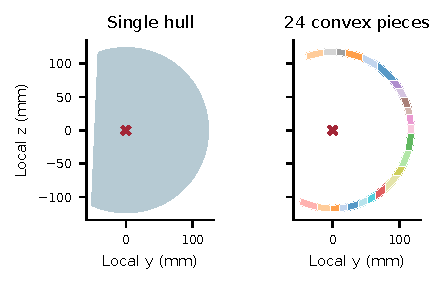
\includegraphics[width=\columnwidth]{collision.pdf}
\caption{Tire collision cross-section from actual mesh data. The single hull (left) fills the cavity. The 24-piece approximation (right) leaves the axle-center probe free while preserving the outer support envelope. Colors distinguish convex pieces; both models retain the same inertial properties.}
\label{fig:collision}
\end{figure}

\section{REWIND-BUDGETED TRAVEL ALLOCATION}
\subsection{Steering and Contact Roles}
For a filtered body command $\vct{c}=[v_x,v_y,\omega_z]^\top$, the required contact travel in the body frame is
\begin{equation}
 \vct{u}_i=-[v_x-\omega_z y_i,\ v_y+\omega_z x_i]^\top,\label{eq:travel}
\end{equation}
where $[x_i,y_i]^\top$ is the nominal contact relative to the footprint centroid. We evaluate both distal rotation signs, clip steering to $\pm35^\circ$, and choose the direction $\hat{\vct{d}}_i$ with greatest alignment to $\vct{u}_i$. A leg qualifies for rolling when the alignment is at least 0.70; fewer than two qualifying legs causes an all-stepping assignment. Under forward motion, this geometry selects legs $\{1,2,5,6\}$ to roll while $\{3,4\}$ step (Fig.~\ref{fig:concept}).

\begin{figure}[t]
\centering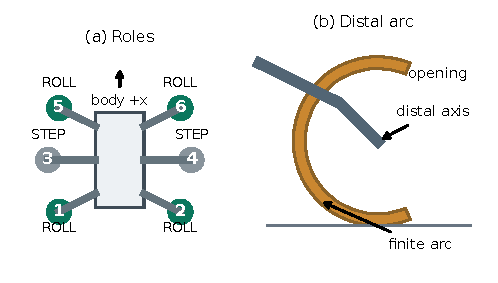
\includegraphics[width=\columnwidth]{concept.pdf}
\caption{Role allocation and finite distal arc, shown schematically. The upper joint changes both rolling heading and foot location. Roles and steering are therefore latched at lift-off. IDs follow the model convention.}
\label{fig:concept}
\end{figure}

\subsection{Rewind Distance and Sector-Rate Bound}
The alternating tripods $\{1,4,5\}$ and $\{2,3,6\}$ have phase offsets of one half-cycle. Frequency $f$ and duty factor $D$ give a swing duration $T_s=(1-D)/f$. A sector rewind from $\theta_{\rm lo}$ to a fixed home $h_i$ uses
\begin{equation}
 \theta(s)=\theta_{\rm lo}+S(s)(h_i-\theta_{\rm lo}),\quad
 S(s)=10s^3-15s^4+6s^5,
\end{equation}
with $s\in[0,1]$. Since $S'(s)=30s^2(1-s)^2$ has maximum $15/8$, a complete swing satisfies $|\dot\theta|\le\Omega$ if
\begin{equation}
 |\theta_{\rm lo}-h_i|\le B,\qquad B=\frac{8}{15}\Omega T_s.\label{eq:budget}
\end{equation}
For $f=2$ Hz, $D=0.60$, and $\Omega=540^\circ$/s, the rewind budget is $B=57.6^\circ$. This is smaller than the geometrically available sector excursion. We use $h_i=0$, which lies in every evaluated sector interval.

During stance, the next sector target is projected into the intersection of its geometric interval and rewind budget:
\begin{equation}
 \theta_{i,k+1}=\Pi_{[\ell_i,u_i]\cap[h_i-B,h_i+B]}
     (\theta_{i,k}+\Delta t\,\omega_{i,k}).\label{eq:project}
\end{equation}
The proposed rate $\omega_{i,k}$ is itself bounded by $\Omega$. For a state already in this interval, projection cannot increase the step magnitude beyond $\Omega\Delta t$. Thus stance respects both the excursion and discrete rate bounds. In swing, we apply an additional projection onto $[\theta_{i,k}-\Omega\Delta t,\theta_{i,k}+\Omega\Delta t]$. This slew guard preserves the discrete sector-rate invariant even when a swing is interrupted or resumed. The complete-swing premise in~\eqref{eq:budget} is required for reaching home within $T_s$; the slew guard alone does not guarantee that endpoint under interruptions.

The budget in~\eqref{eq:budget} is specific to the selected quintic profile, not the maximum recoverable angle for every trajectory. A constant-speed return would have a different factor and different endpoint smoothness. For a geometric reserve $A_i$ about home, the usable excursion is $\min(A_i,B)$. Thus the temporal constraint becomes active when $15A_i/(8\Omega T_s)>1$. This criterion describes where a geometric limit is insufficient; it does not prove contact stability or IK reachability.

A rolling leg decides whether to reindex at swing-window entry, based on spent reserve, loss of alignment, or predicted exhaustion before its next opportunity. For a locally constant sector rate, skipping the current window predicts $\theta_i^+=\theta_i+\omega_i/f$. If this value lies outside the intersection in~\eqref{eq:project}, the leg reindexes now. This one-cycle lookahead is a scheduling heuristic under changing commands, while the excursion and slew bounds remain explicit. This avoids starting a quintic trajectory midway through its allotted window. Roles are updated at actual lift-off. A stepping leg uses every swing window; rolling legs can skip unneeded swings. The schedule leaves at least three legs commanded in stance, while the number of loaded contacts is measured separately.

\subsection{Allocation After Saturation}
Before angular projection, the requested rolling speed is the projection of contact travel onto the steered rolling direction, scaled by an authority $\beta_i$. Authority fades over the last $12^\circ$ of the geometric interval. After~\eqref{eq:project}, articulation receives the residual based on the increment that will actually be commanded:
\begin{equation}
 \vct{u}^{\rm art}_i=\vct{u}_i-
 s_i r_i\frac{\theta_{i,k+1}-\theta_{i,k}}{\Delta t}\hat{\vct{d}}_i,\label{eq:residual}
\end{equation}
where $s_i$ maps the selected motor sign to rolling direction. This subtraction prevents the walking trajectory from requesting travel already assigned to rotation. Using the pre-saturation request would leave an unaccounted residual once the rewind budget is exhausted.

The residual is integrated into a stance offset, bounded by a 90/70 mm longitudinal/lateral elliptical workspace. Numerical IK generates articulated targets with a $40^\circ$ distal-branch guard and stride backoff when needed. The sector offset is added to the distal target, and final targets are clipped to $[0^\circ,360^\circ]$. The allocation equality describes commanded kinematics before workspace and final motor clipping; tracking lag and slip need not satisfy it. In particular, the summed distal target contains both IK and sector motion. The sector-rate invariant is not a bound on that sum. Before final clipping, $q^\star_{3,i}=q^{\rm IK}_{3,i}+\theta_i$. A physical target-rate constraint would require
\begin{equation}
 |\Delta q^{\rm IK}_{3,i}+\Delta\theta_i|\le\dot q_{3,i}^{\max}\Delta t.\label{eq:joint}
\end{equation}
A sufficient bound is $|\Delta q^{\rm IK}_{3,i}|+|\Delta\theta_i|\le\dot q_{3,i}^{\max}\Delta t$. This coupled constraint is not enforced by the evaluated allocator; the recorded total target rates quantify that limitation.



\section{EXPERIMENTAL METHOD}
\subsection{Common Protocol and Restrictions}
We use MuJoCo 3.10.0~\cite{todorov2012mujoco}, a 2 ms physics step, and a 20 ms command update. Each fresh model is initialized, placed at the common nominal pose, and settled for 1 s before an 8 s measurement. The 0.15 s command filter and initial role-adoption transient are included. The maximum step height is 25 mm. There is no parameter retuning across conditions.

The main matrix compares the seven conditions in Table~\ref{tab:conditions} at forward commands of 0.18 and 0.45 m/s and initial phases $k/8$, $k=0,\ldots,7$, giving 112 trials. The primary geometry is the decomposed arc. U is the pre-guard travel allocator, while B adds the budget, fixed home, swing-entry decision, next-window lookahead, and slew guard together. Their comparison tests this complete rewind treatment, not an isolated projection operator. G removes the lookahead and tests whether a bounded excursion alone suffices for a reachable residual trajectory. The other restrictions retain B's settings.

\begin{table}[t]
\caption{Controller restrictions in the main comparison}
\label{tab:conditions}\centering\small
\begin{tabular}{cp{6.7cm}}\toprule
Code & Definition\\\midrule
U & Original allocation; geometric arc limits, original swing timing.\\
B & Proposed rewind-budgeted allocation.\\
G & B without the next-window budget lookahead.\\
N & B with all rolling roles disabled.\\
S & B with full articulated travel superposed on rolling; no subtraction.\\
D & B with rolling-leg reindexing disabled after role adoption.\\
P & B with periodic rolling-leg swings at every window.\\\bottomrule
\end{tabular}
\end{table}

An additional 84 trials compare B/N/S over seven commands: forward 0.30 m/s, reverse $-0.18$ m/s, lateral $\pm0.12$ m/s, yaw $\pm0.45$ rad/s, and a curve at 0.18 m/s with 0.35 rad/s yaw. Each uses four phases. Three separate stress settings---mass multiplied by 1.2, friction by 0.5, or actuator strength by 0.8---yield 36 high-command trials of B/N/S over four phases. These factors are declared numerical stress cases, not identified hardware uncertainty distributions.

We further repeat B/N/S on the single-hull geometry at both main commands and four phases (24 trials). Timestep checks use 1 and 4 ms at the high command and phases 0 and 0.5 (12 trials), paired with the existing 2 ms records. The complete design therefore contains 268 trials. The commands are constant within each trial; they do not establish closed-loop command-transition performance.

The source revision, dependencies, model and decomposition hashes, condition matrix, and output rules are fixed before the complete run. Raw failures are retained. A target rejected by the public sender because IK did not converge terminates its trial, as do nonfinite state and a body tilt exceeding $60^\circ$. Completion is reported independently of tracking accuracy. A development run exposed premature budget exhaustion without lookahead; this motivated B and the explicit G restriction. The reported matrix was then frozen and run in full. It is a confirmation of the revised mechanism, not an independently held-out benchmark. Earlier development results are not pooled with these summaries.

\begin{table*}[t]\centering\small
\caption{Main matrix: completion and full-window speed, mean [minimum, maximum]}
\label{tab:main}
\begin{tabular}{ccccccc}\toprule
 & \multicolumn{2}{c}{0.18 m/s command} & \multicolumn{2}{c}{0.45 m/s command} & \multicolumn{2}{c}{High-command peak rate ($^\circ$/s)}\\
Code & Complete & Speed (m/s) & Complete & Speed (m/s) & Sector & Total distal\\\midrule
U & 8/8 & 0.114 [0.113, 0.116] & 8/8 & 0.283 [0.278, 0.288] & 1516.8 & 3299.5\\
B & 8/8 & 0.114 [0.113, 0.116] & 8/8 & 0.283 [0.280, 0.286] & 536.4 & 1405.5\\
G & 8/8 & 0.114 [0.113, 0.116] & 0/8 & -- & 535.7 & 1291.9\\
N & 8/8 & 0.094 [0.092, 0.095] & 8/8 & 0.126 [0.122, 0.129] & 0.0 & 1763.2\\
S & 0/8 & -- & 0/8 & -- & 179.3 & 1301.6\\
D & 0/8 & -- & 0/8 & -- & 203.0 & 1291.9\\
P & 8/8 & 0.113 [0.111, 0.114] & 8/8 & 0.284 [0.281, 0.285] & 536.4 & 1191.8\\
\bottomrule\end{tabular}
\par\vspace{5pt}\noindent\parbox{.96\textwidth}{\footnotesize Total distal denotes IK plus sector target; the sector bound does not apply to it. Peaks for failed conditions cover only the interval before termination. A dash indicates that no trial completed the full 8 s; truncated speeds are not averaged into successful performance.}
\end{table*}

\subsection{Metrics}
Primary forward transport is the net displacement projected onto the initial chassis axis, divided by the measured duration. A world-frame velocity integral at the same root origin provides an independent cross-check in 20 separate validation replays. Translational and yaw-rate RMSE compare instantaneous body-frame motion with the original command, including startup transients. Failed trials have shorter durations and are reported as failures; their truncated speeds are not substituted for full-window averages.

We measure sector-command peak rate, peak excursion, and the number of command frames exceeding the 540 degree/s sector limit. We separately record the rate of the summed distal motor target from successive measurement commands, excluding the first command for which that recorder has no previous target. The additional analysis of this metric is post hoc; it reuses the frozen records without adding trials. Loaded-leg count uses distinct tire bodies with normal contact force above 1 N, so subdividing a tire cannot create additional counted legs.

Absolute mechanical work is $W_{\rm abs}=\int\sum_{j=1}^{18}|\tau_j\dot q_j|dt$. Its transport normalization is $W_{\rm abs}/(mg\|\Delta\vct{p}_{xy}\|)$, using net planar displacement. This quantity is not battery energy. Slip integrates mean tangential velocity over loaded tire--ground contact points; it is neither load weighted nor independent of collision-point multiplicity. We consequently compare slip primarily within one geometry.

Phases are a deterministic grid rather than independent random samples. We report means, full observed ranges, and phase-paired differences without population confidence intervals. Positive transport or survival of the tilt threshold is insufficient evidence of reliable operation.

\section{RESULTS}
\subsection{Rewind Feasibility and Forward Transport}
The rewind treatment preserves forward transport while reducing sector demand. At the 0.45 m/s command, B retains 99.95\% of U's mean speed and reduces the largest sector-command rate from 1516.8 to 536.4 degree/s (Table~\ref{tab:main}). Both complete all eight phases; U exceeds the prescribed sector rate in every high-command trial, whereas B has no violating frames. The small speed difference is an observed difference, not a statistical equivalence claim. Figure~\ref{fig:rate} shows the phase-zero sector trajectories.



\begin{figure*}[t]
\centering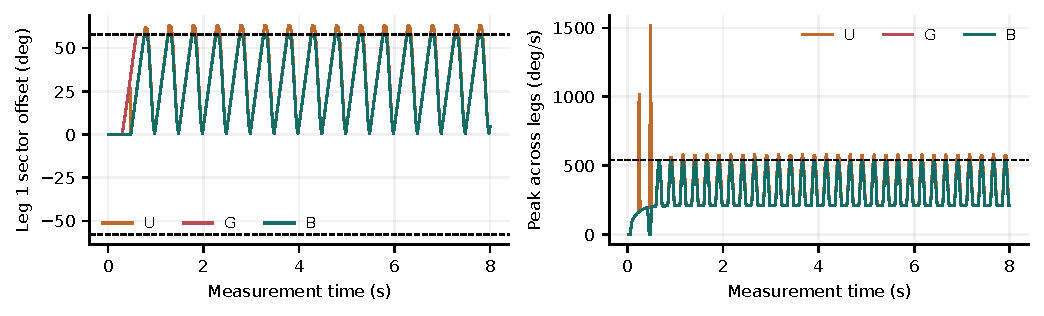
\includegraphics[width=.97\textwidth]{rate_budget.pdf}
\caption{Sector allocation in phase-zero, high-command trials. Left: leg-1 sector trajectories for U, B, and G; the G trace ends when its trial terminates. Right: maximum absolute sector rate across the six legs, with the prescribed 540 degree/s limit. These traces show the sector component of the command, before addition to the articulated distal target.}
\label{fig:rate}
\end{figure*}



The distance-only restriction G completes the low-command trials but rejects an IK target in all eight high-command trials. Bounding sector excursion without anticipating the next swing can exhaust the rolling budget while the leg remains in stance; the resulting articulated residual becomes unreachable. Adding the lookahead in B restores completion for these trials. The full-superposition restriction S and disabled-reindexing restriction D reject targets in all main trials. These outcomes concern this posture, workspace, and command range; they do not imply that all superposed or nonreindexing controllers must fail.

Periodic P also completes all main trials and attains 0.284 m/s at the high command, compared with B's 0.283 m/s. The phase-paired B-minus-P speed differences span $[-0.00255,0.00060]$ m/s. At the low command, B has only a small mean advantage. These observations support timely reindexing without establishing adaptive scheduling as superior to periodic scheduling.

A post-hoc comparison of the recorded summed distal targets gives additional context. The largest high-command target rate decreases from 3299.5 degree/s for U to 1405.5 degree/s for B, a 57.4\% reduction of the worst observed value. Six phase-paired peaks decrease and two remain unchanged to numerical tolerance. However, P has a smaller maximum of 1191.8 degree/s. These target derivatives are not measured motor speeds, and neither B nor P satisfies a 540 degree/s bound on the total target.

Disabling rolling in N reduces mean forward speed to 0.126 m/s. The B-minus-N gain averages 0.157 m/s and spans [0.151, 0.162] m/s across paired phases, yielding a mean speed ratio of 2.25. This is a within-family restriction comparison; N was not independently optimized for walking.

\begin{figure*}[t]\centering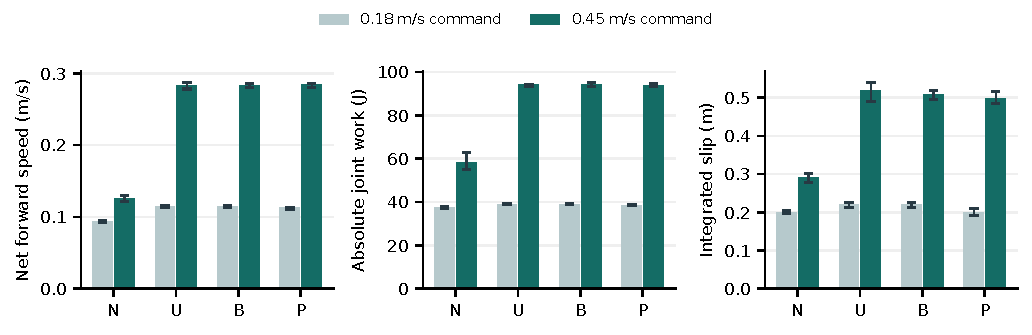
\includegraphics[width=.97\textwidth]{results.pdf}
\caption{Four conditions that complete every main trial. Bars are eight-phase means; whiskers are full phase ranges. G, S, and D are reported with their failures in Table~\ref{tab:main}. Faster transport is accompanied by changes in joint work and slip, so speed alone is not an efficiency result.}
\label{fig:results}\end{figure*}
\subsection{Work, Tracking, and Loaded Support}
At the high command, B uses 94.2 J of absolute joint work against N's 58.1 J. Integrated slip is 0.509 versus 0.290 m. Their respective translational RMSE values are 0.196 and 0.331 m/s. B therefore improves net transport without demonstrating uniformly lower work or slip. Its main trials include a minimum loaded-leg count of 1, and up to 11.65\% of physics samples have fewer than three. This illustrates why a three-leg stance schedule is not a three-contact load guarantee. Across all 68 B trials, the summed distal target reaches 1594.6 degree/s; the 1405.5 degree/s value in Table~\ref{tab:main} covers only the main high-command subset. Applying the method to a physical actuator requires a joint-level trajectory constraint.

\subsection{Commands Beyond Forward Motion}
Table~\ref{tab:domain} reports all seven additional commands. Translational and yaw errors are separate because a controller can remain upright while tracking poorly. Each comparison uses the same four initial phases. The results describe constant-command operating points, including cases where both B and N fall back to stepping.
\begin{table*}[t]\centering\small
\caption{Additional commands: completion and tracking error over completed trials}
\label{tab:domain}\begin{tabular}{lccccc}\toprule
Command $(v_x,v_y,\omega_z)$ & Complete B/N/S & B $e_v$ & N $e_v$ & B $e_\omega$ & N $e_\omega$\\\midrule
(0.3, 0, 0) & 4/4/0 & 0.124 & 0.177 & 0.084 & 0.086\\
(-0.18, 0, 0) & 4/4/0 & 0.078 & 0.097 & 0.058 & 0.036\\
(0, 0.12, 0) & 4/4/4 & 0.041 & 0.057 & 0.004 & 0.002\\
(0, -0.12, 0) & 4/4/4 & 0.042 & 0.057 & 0.005 & 0.002\\
(0, 0, 0.45) & 4/4/4 & 0.043 & 0.043 & 0.275 & 0.275\\
(0, 0, -0.45) & 4/4/4 & 0.042 & 0.042 & 0.274 & 0.274\\
(0.18, 0, 0.35) & 4/4/1 & 0.102 & 0.112 & 0.186 & 0.212\\
\bottomrule\end{tabular}
\par\vspace{5pt}\noindent\parbox{.96\textwidth}{\footnotesize Each completion count is out of four. $e_v$ is translational RMSE (m/s); $e_\omega$ is yaw-rate RMSE (rad/s). Units of the command are m/s, m/s, and rad/s. Failed-trial errors are not mixed with full-window errors.}
\end{table*}

\subsection{Parameter, Geometry, and Timestep Checks}
With 1.2-fold mass, B completes 4/4 trials and N completes 4/4. Their mean speeds are 0.270 and 0.118 m/s. With half nominal friction, B completes 4/4 trials and N completes 4/4. Their mean speeds are 0.316 and 0.134 m/s. With 0.8-fold actuator strength, B completes 4/4 trials and N completes 4/4. Their mean speeds are 0.293 and 0.130 m/s. These isolated stress cases are not a population robustness estimate.

For paired completed B/N trials, changing from decomposed contacts to the single hull changes net speed by at most 0.0122 m/s. The 1/2/4 ms comparison changes speed by at most 0.0008 m/s relative to 2 ms. These are local sensitivity results, not a proof of solver convergence or concave-edge accuracy. Contact-point slip is not compared across the two representations because decomposition changes the contact manifold.

Across the prescribed matrix, 193/268 trials complete; all incomplete trials terminate because an IK target is rejected. B completes 68/68 trials with 0 sector-rate violation frames. A separate 20-trial check integrates the velocity at the same root origin used for displacement. Its maximum speed discrepancy is 0.00009 m/s. Velocity at the body center of mass is retained as a diagnostic at a different point and is not substituted for velocity at the root origin. The three visual replays in Fig.~\ref{fig:replay} reproduce the corresponding nominal records to the verified numerical tolerance.


\begin{figure*}[t]
\centering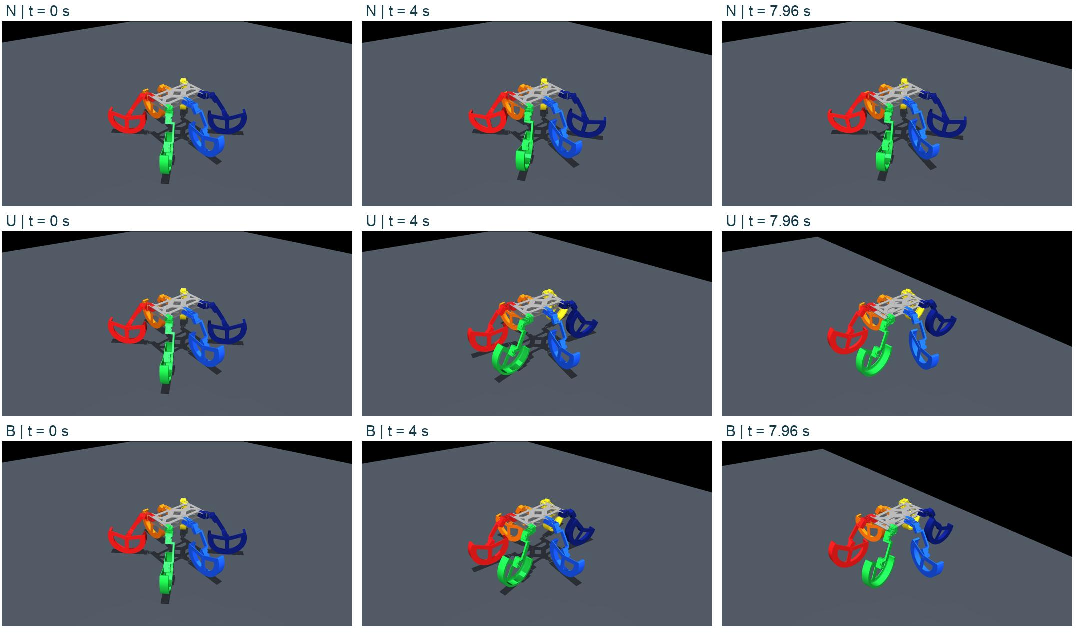
\includegraphics[width=.97\textwidth]{replay.pdf}
\caption{Actual simulation replays at the high command, phase zero, using decomposed tire contacts. Rows show N, U, and B; columns show measurement times 0, 4, and 7.96 s. The camera follows the robot; speed is measured from model state. The colors show model components, not contact force. All replays are checked against the corresponding raw record.}
\label{fig:replay}
\end{figure*}

\section{DISCUSSION}
\subsection{What the Comparison Establishes}
The main result is reduced rewind demand at nearly unchanged transport relative to U. Both methods roll on the same articulated robot, so this contrast addresses the cost of adding a rewind constraint. The comparison with N answers a separate question: how much rolling contributes within this fixed gait family. It does not compare against an optimized walking controller. G, S, and D diagnose implementation mechanisms; their failures are rejected IK targets, not observed hardware falls.

Periodic P is the strongest simple alternative in the main matrix. It attains comparable speed and a smaller largest summed distal-target rate than B. The present evidence therefore does not justify choosing adaptive scheduling for better speed, energy, or actuator demand. The transferable design lesson is to coordinate rewind time and residual travel, while the choice between periodic and adaptive reindexing remains application dependent. Direct comparisons with a joint-constrained planner and external methods are needed to establish a broader performance advantage.

\subsection{Limits of the Guarantee and the Model}
The sector-rate invariant applies to a component of the target, not to measured actuator motion. Equation~\eqref{eq:joint} identifies the additional coupling required for a full joint-rate bound. The observed reduction in total target rate is encouraging but does not satisfy that requirement. The $540^\circ$/s setting is a declared simulation budget, not an identified hardware limit. The current planner also lacks force optimization and a loaded-support guarantee.

The study covers constant commands, eight-second windows, one nominal morphology, and selected parameter perturbations. It does not establish long-duration reliability, terrain generalization, command-transition robustness, or parameter uncertainty identified from hardware. The contact decomposition preserves the arc cavity, but the tire remains rigid; most link and motor collision geoms are disabled, and hinge hard stops are absent. These assumptions limit claims about collision clearance, compliant contact, and physical feasibility.

Archival floor and stair recordings document the prototype's physical embodiment. They lack synchronized control logs and repeated measurements for B, and cannot validate the new allocator. Figure~\ref{fig:platform} provides this context; the accompanying video also retains the historical stair sequence with explicit labeling. A decisive next test is a matched comparison of B, U, and periodic P under measured joint limits, followed by synchronized pose, joint, and current measurements on the prototype.

\section{CONCLUSION}
A finite arc's usable rolling excursion depends on the time available for its next rewind. We coupled this swing-time budget to residual contact-travel allocation on an articulated hexapod. In the prescribed simulation study, the method reduced sector-command peaks while retaining the original allocator's forward transport. A distance bound alone was insufficient in the high-command cases, while periodic reindexing remained competitive. These findings support the mechanism in simulation; joint feasibility and hardware validation remain open.

\noindent\begin{minipage}{\columnwidth}
\section*{ACKNOWLEDGMENT OF AI ASSISTANCE}
OpenAI Codex assisted with the Abstract, Sections I--VIII, source analysis, controller and evaluation code, and figure and video assembly. Numerical observations came from executed simulations or geometry calculations, and physical images from archival recordings. The generated material was checked against the recorded simulations, source files, and cited sources during manuscript preparation.
\end{minipage}
\par
\interlinepenalty=10000
\IEEEtriggeratref{7}\bibliographystyle{IEEEtran}\bibliography{references}
\end{document}
